%% Tex spellcheck = fr_FR
\chapter*{Introduction}
\addcontentsline{toc}{chapter}{Introduction} % Adding toc entry

As the final step in our Bachelor's program in Computing and Communication Systems at \gls{hepia}, we undertake a Bachelor project that spans 14 weeks immediately following our last semester. It extends for a period of 14 weeks during which a workload of 450 hours is expected. This project is the culmination of our studies and is intended to demonstrate our ability to apply the knowledge and skills acquired during our studies to a concrete problem.

% Project is a magnetic tic tac toe
Our initial project concept was to design and implement a \gls{pcb}-based chessboard, where chess pieces are moved using magnetic fields generated by electromagnets directly etched onto the \gls{pcb}. However, due to the complexity involved in implementing, producing, shipping, and using a chessboard of this nature, we decided to shift our focus to another board game—Tic-Tac-Toe—that shares similar concepts but offers a more manageable form factor. Should there be a need, the project can be scaled up to a chessboard with minimal adjustments, extending the board and reprogramming the game rules.

Tic-Tac-Toe is a simple game played on a 3x3 grid, where two players take turns placing their pieces on the board. The objective is to be the first to align three pieces in a row, column, or diagonal. Our implementation of this game eliminates the need for physical interaction with the board. The pieces, embedded with magnets, are moved by electromagnets that are etched onto the \gls{pcb}.

\begin{figure}[H]
	\centering
	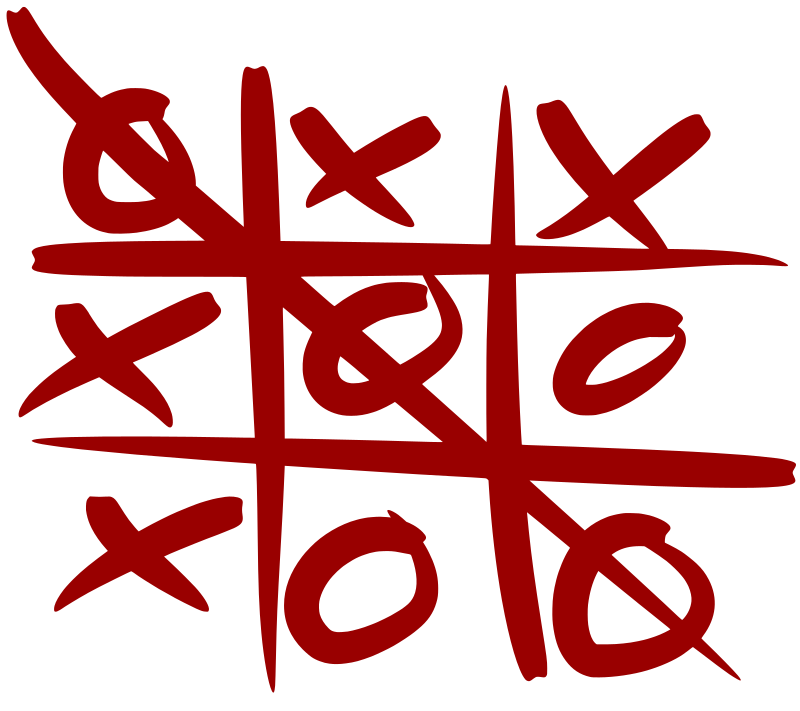
\includegraphics[width=0.5\linewidth]{tic_tac_toe.png}
	\caption[Tic Tac Toe example]{Tic Tac Toe example}
	\label{fig:tictactoe_game}
\end{figure}

Players interact solely through a web application, which displays the game board and enables them to make their moves. This application communicates with a backend, which in turn connects to a microcontroller responsible for controlling the electromagnets. The microcontroller activates the coils in a specific sequence to move the pieces on the board.

% Why this project
The project was chosen because it combines several aspects of our studies, such as electronics, software development and microcontroller programming. It also allows us to work on a project from start to finish, from the design phase to the implementation and testing phase. The project is also interesting because it involves the use of different technologies as \gls{pcb} design, microcontroller programming, and web development.

% Objectives
The primary objective of this project is to design and implement a functional, automated Tic-Tac-Toe board that utilizes electromagnetism to move the pieces, completely eliminating the need for manual interaction. While the project focuses on a simple game like Tic-Tac-Toe, it serves as a proof of concept for more complex games such as chess. In a chess setting, this technology could enable spectators to watch a grandmaster's game with the moves being replicated in real-time on a physical board, without anyone needing to physically move the pieces. Or it could be used for educational purposes, allowing students to play against a computer that moves the pieces for them.

% Structure
This thesis is organized into three main sections, each addressing a distinct aspect of the project. The first section explores the theoretical concepts of magnetism and electromagnetism, along with simulations conducted to validate the concept. The second section focuses on the iterative design process of the hardware to identify the optimal coil design. The third section details the final hardware design and the software components of the project.